\documentclass[tikz,border=2pt]{standalone}
\usepackage{amsmath,amssymb}
\usepackage{tikz}

\begin{document}
% The four bounded intervals with endpoints a<b: a filled dot means the endpoint belongs to the
% interval, an open dot means it does not.
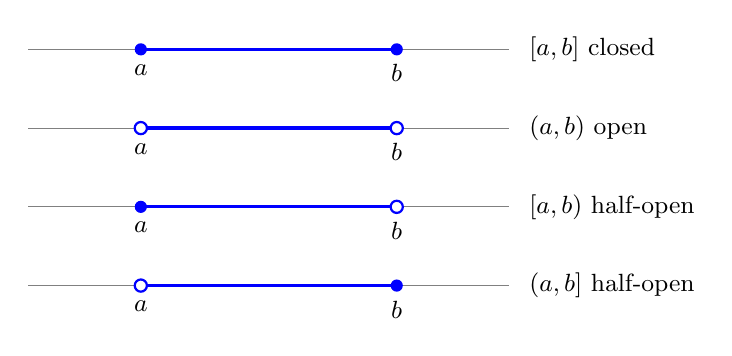
\begin{tikzpicture}[x=1.3cm, every node/.style={font=\small}]
	\foreach \y/\lab/\left/\right in {0/{$[a,b]$ closed}/fill/fill, -1/{$(a,b)$ open}/open/open, -2/{$[a,b)$ half-open}/fill/open, -3/{$(a,b]$ half-open}/open/fill} {
		\draw[gray] (-0.6,\y) -- (4.1,\y);
		\draw[very thick, blue] (0.5,\y) -- (3,\y);
		\node[anchor=west] at (4.2,\y) {\lab};
		\node[below=2pt] at (0.5,\y) {$a$};
		\node[below=2pt] at (3,\y) {$b$};
	}
	\fill[blue] (0.5,0) circle (2.2pt);  \fill[blue] (3,0) circle (2.2pt);
	\draw[blue, thick, fill=white] (0.5,-1) circle (2.2pt); \draw[blue, thick, fill=white] (3,-1) circle (2.2pt);
	\fill[blue] (0.5,-2) circle (2.2pt); \draw[blue, thick, fill=white] (3,-2) circle (2.2pt);
	\draw[blue, thick, fill=white] (0.5,-3) circle (2.2pt); \fill[blue] (3,-3) circle (2.2pt);
\end{tikzpicture}
\end{document}
